\section{Flux Inputs and Uncertainties}\label{sec:nu-osc-05}
%{\it Assigned to:} {\bf Laura Fields} with contributions from Zarko Pavlovic and Luke Pickering.
\label{sec:physics-lbnosc-flux}

The neutrino fluxes are described in detail in Section~\ref{sec:tools-mc-flux}.  They were generated using G4LBNF, a \textsc{Geant}4\xspace-based simulation of the LBNF neutrino beam.  The simulation was configured to use a detailed description of the LBNF optimized beam design~\cite{optimizedbeamcdr}, which includes horns and target designed to optimize sensitivity to CP violation.   

\begin{dunefigure}[Neutrino fluxes at the far detector]{fig:flux_flavor}
{Neutrino fluxes at the far detector for neutrino mode (left) and
antineutrino mode (right). }
    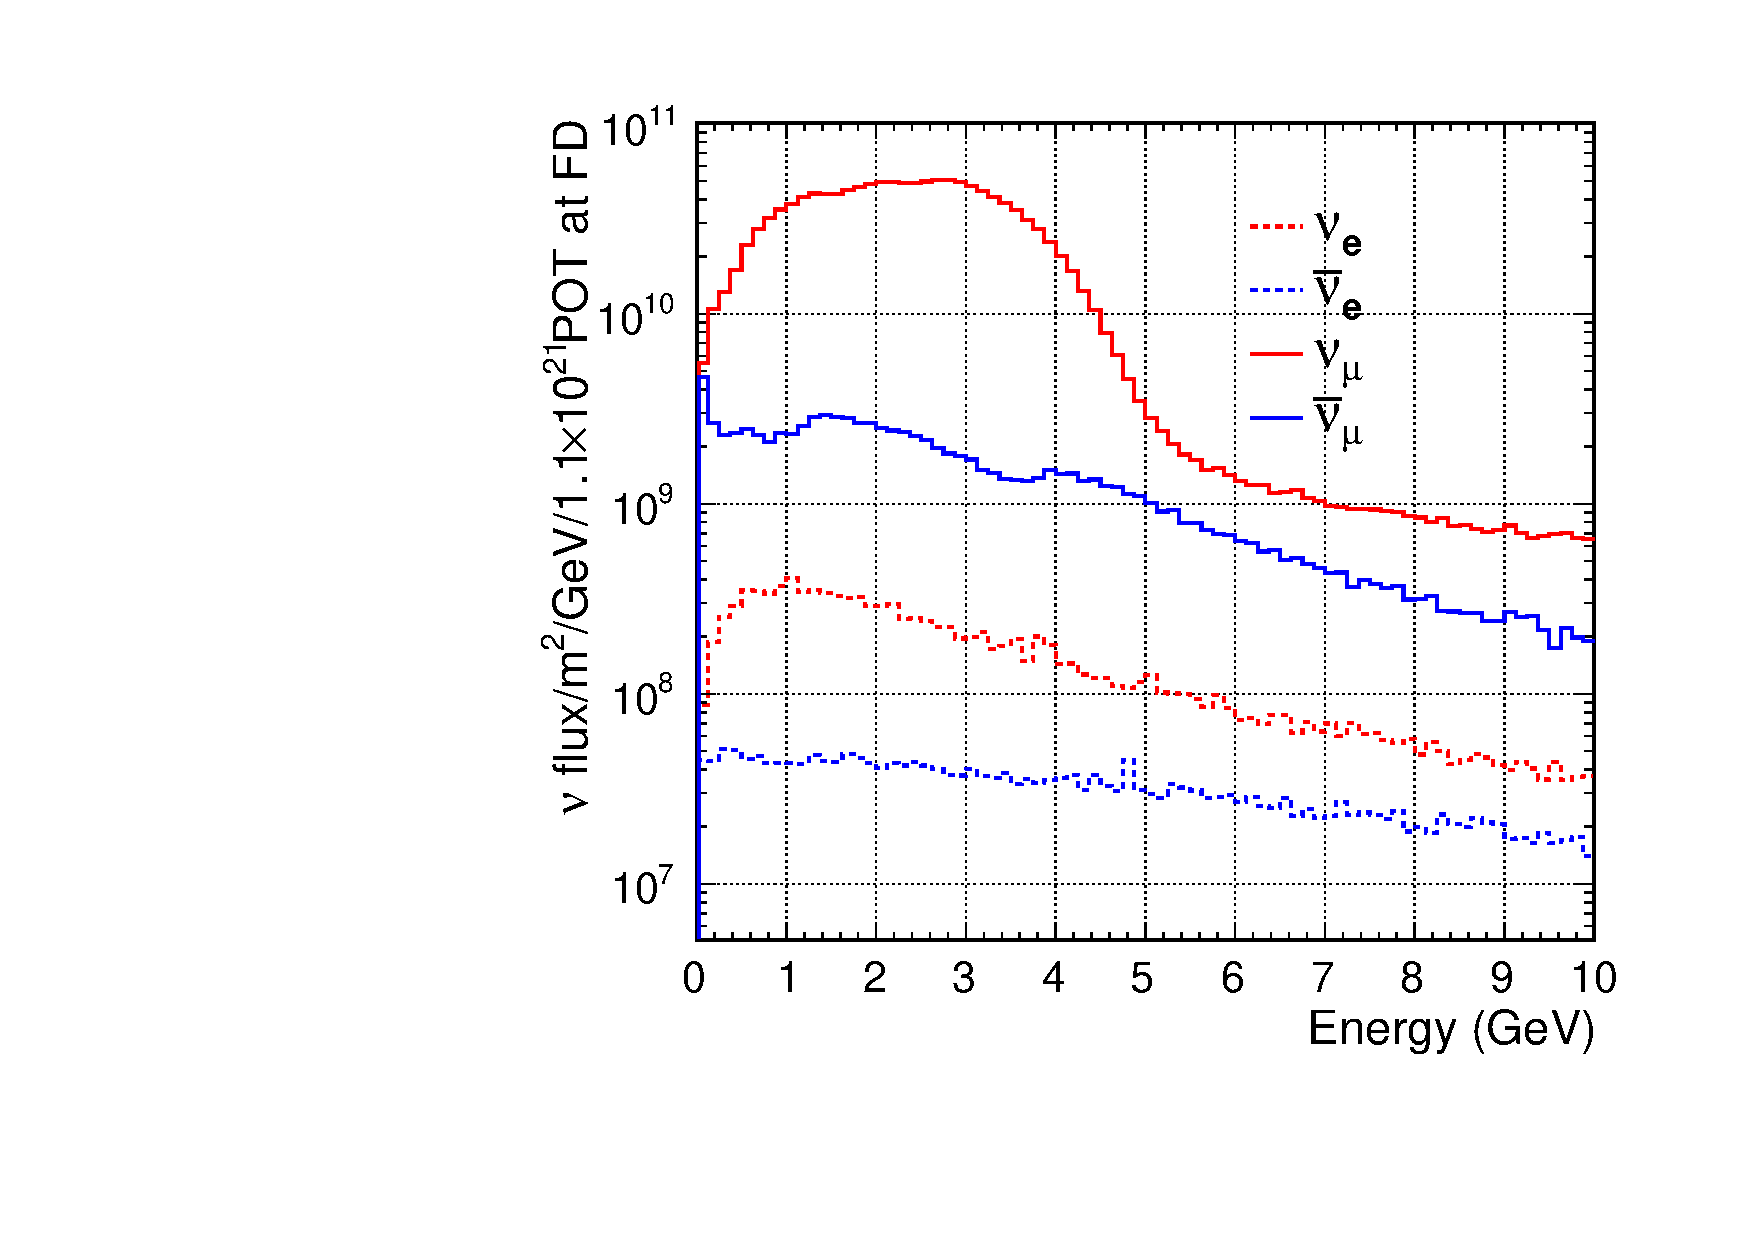
\includegraphics[width=0.45\textwidth]{graphics/dune_neutrino_fd_log.pdf}
     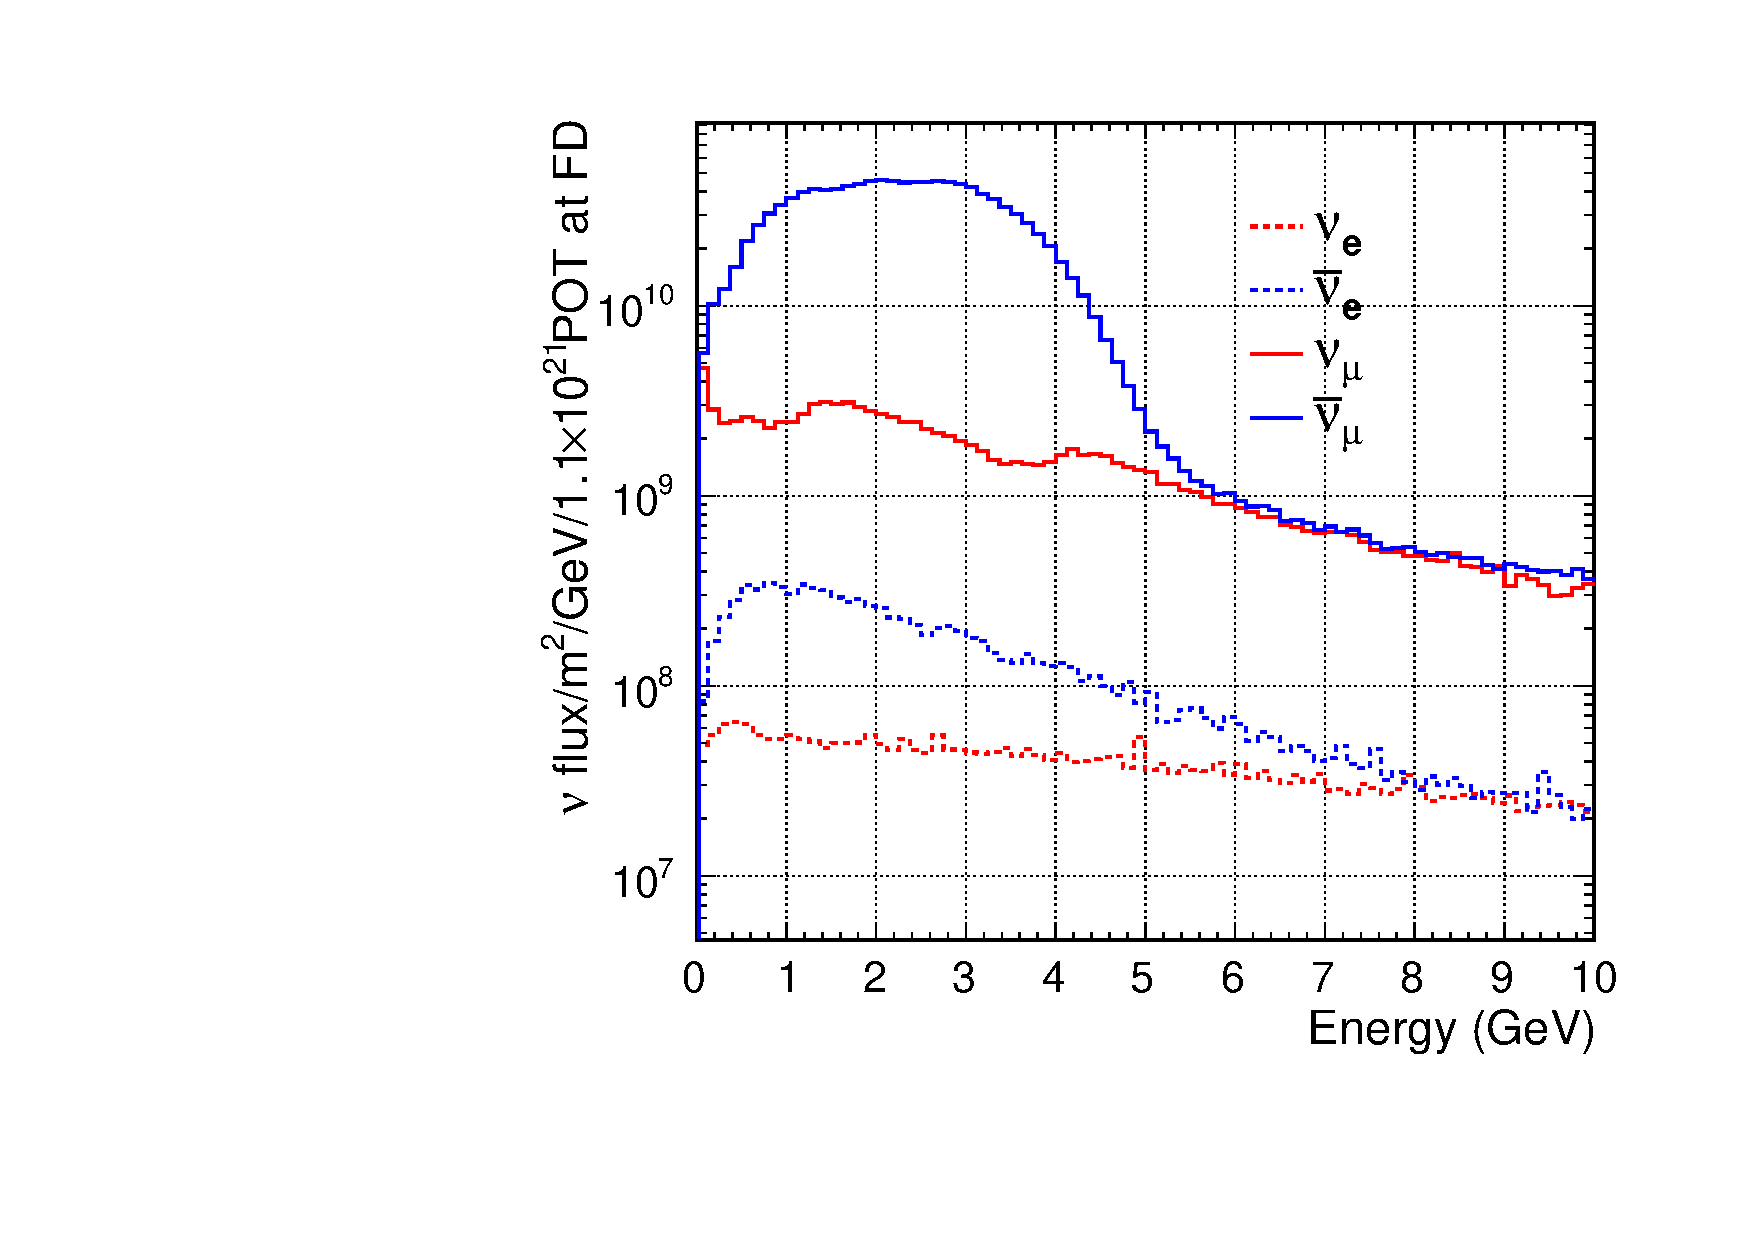
\includegraphics[width=0.45\textwidth]{graphics/dune_antineutrino_fd_log.pdf}
\end{dunefigure}

Neutrino fluxes for neutrino and antineutrino mode configurations of LBNF are shown in Figure~\ref{fig:flux_flavor}.   Uncertainties on the neutrino fluxes arise primarily from uncertainties in hadrons produced off the target and uncertainties in parameters of the beam such as horn currents and horn and target positioning (commonly called "focusing uncertainties"). Given current measurements of hadron prodution and LBNF estimates of alignment tolerances, these lead to uncertainties of approximately 8\% at the first oscillation maximum and 12\% at the second, and are highly correlated between energy bins and across neutrino flavors.       

The fluxes at the near and far detector are similar, but not identical.  Flux uncertainties mostly cancel for the ratio of fluxes between the two detectors.  Uncertainties on the ratio are around 1\% or smaller except at the falling edge of the focusing peak, where they rise to 2\%.    

The neutrino flux spreads beyond the beam directly aimed at the DUNE Far Detector and viable neutrino fluxes extend outward at the near detector hall. The relationship between the parent pion energy and neutrino energy is shown in Fig.~\ref{fig:OAAFluxFigs}; for an ``off-axis'' angle relative to the initial beam direction, the subsequent neutrino energy spectra is narrower and peaked at a lower energy than the on-axis spectra. At $575\,\textrm{m}$, the location of the near detector hall, a lateral shift of $1\,\textrm{m}$ corresponds to approximately a $0.1^\circ$ change in off-axis angle.

\begin{dunefigure}[optional caption for LoF]{fig:OAAFluxFigs}
{(a) The neutrino energy as a function of parent pion energy for different angles away from the pion momentum vector. Figure from Ref.~\cite{Duffy:2016owt}. (b) The DUNE near detector flux predictions over a range of off-axis positions for a near detector at $575\,\textrm{m}$ downstream of the target station. }
%is subfig package included? I don't think subfloat is working (ZP)
%  \subfloat[C][Off-axis pion decay kinematics]{
    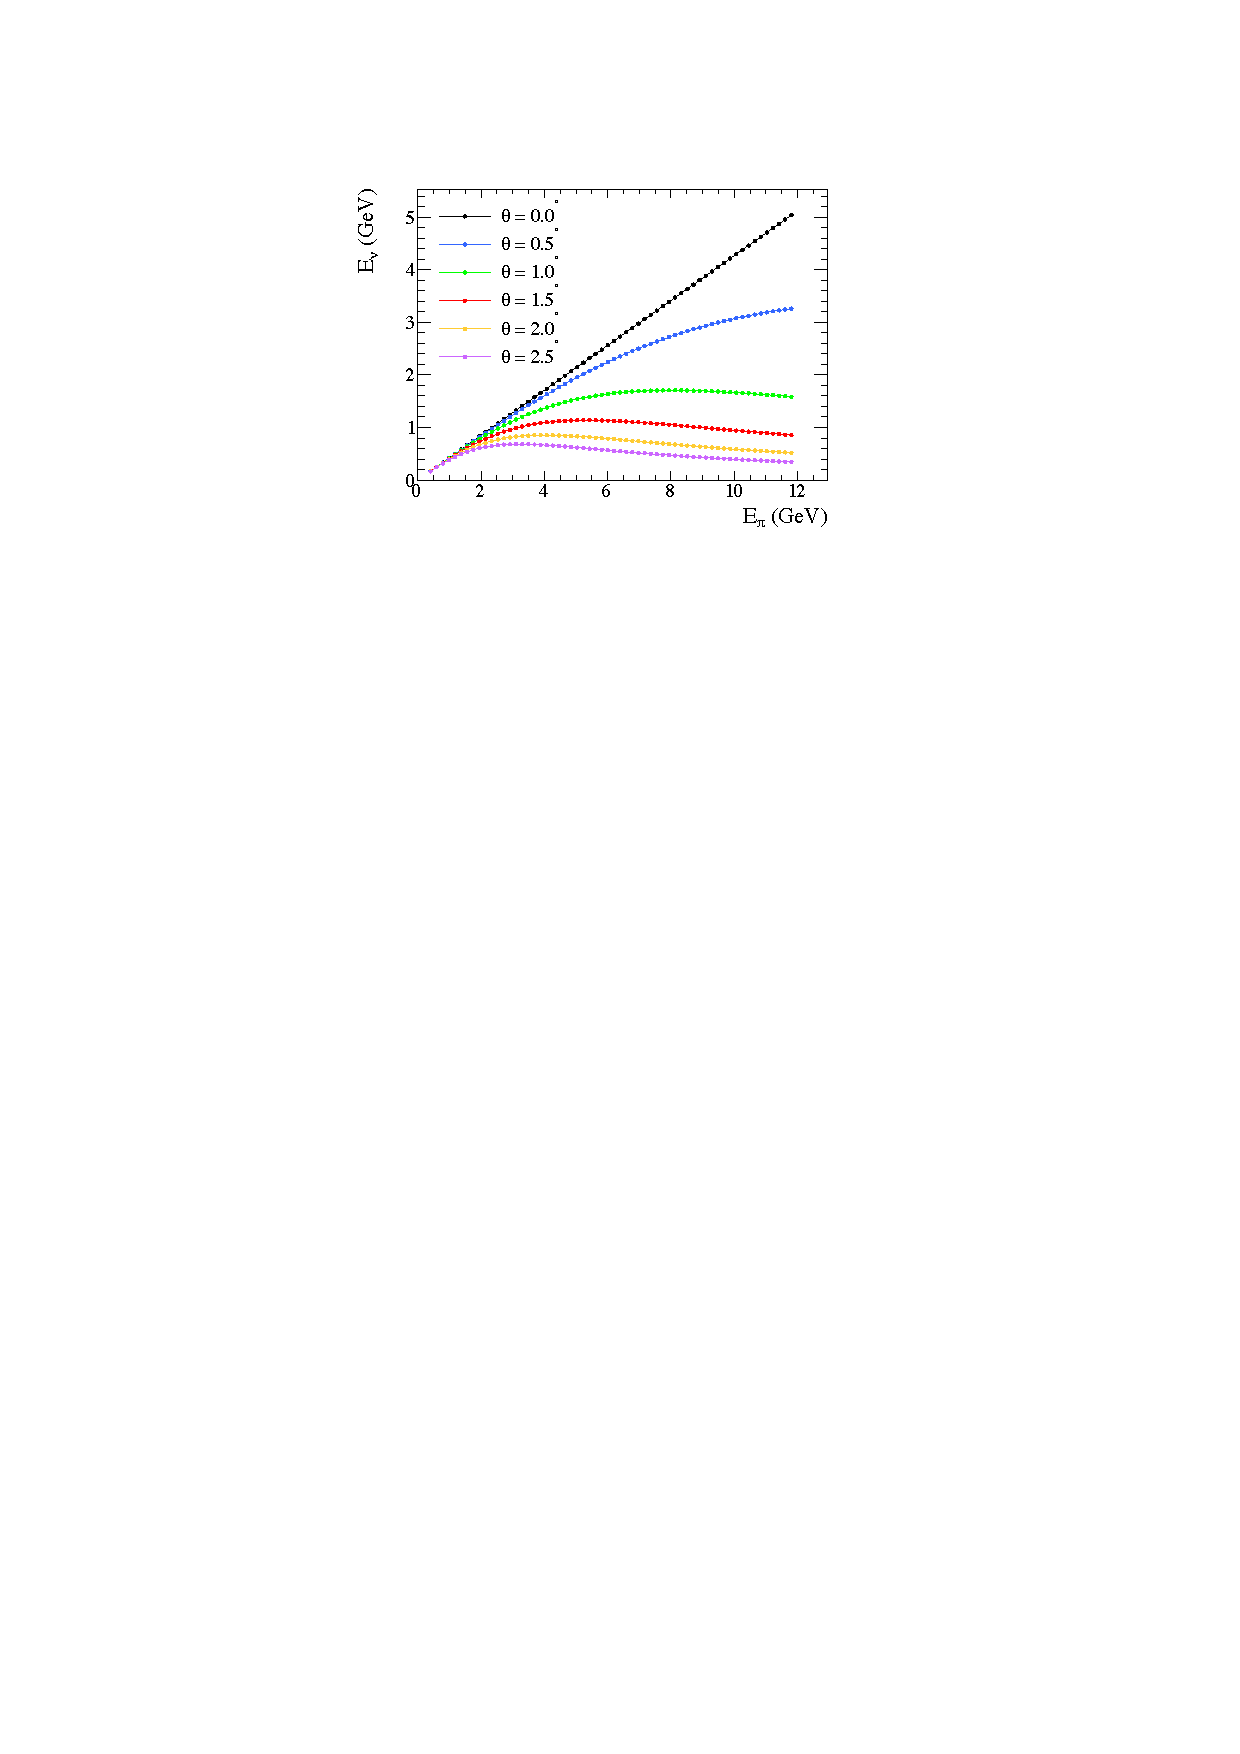
\includegraphics[width=0.4\textwidth]{OATrick}
%    \label{fig:OATrick}
%  }
%  \subfloat[][DUNE near detector flux predictions]{
    \raisebox{0.5em}{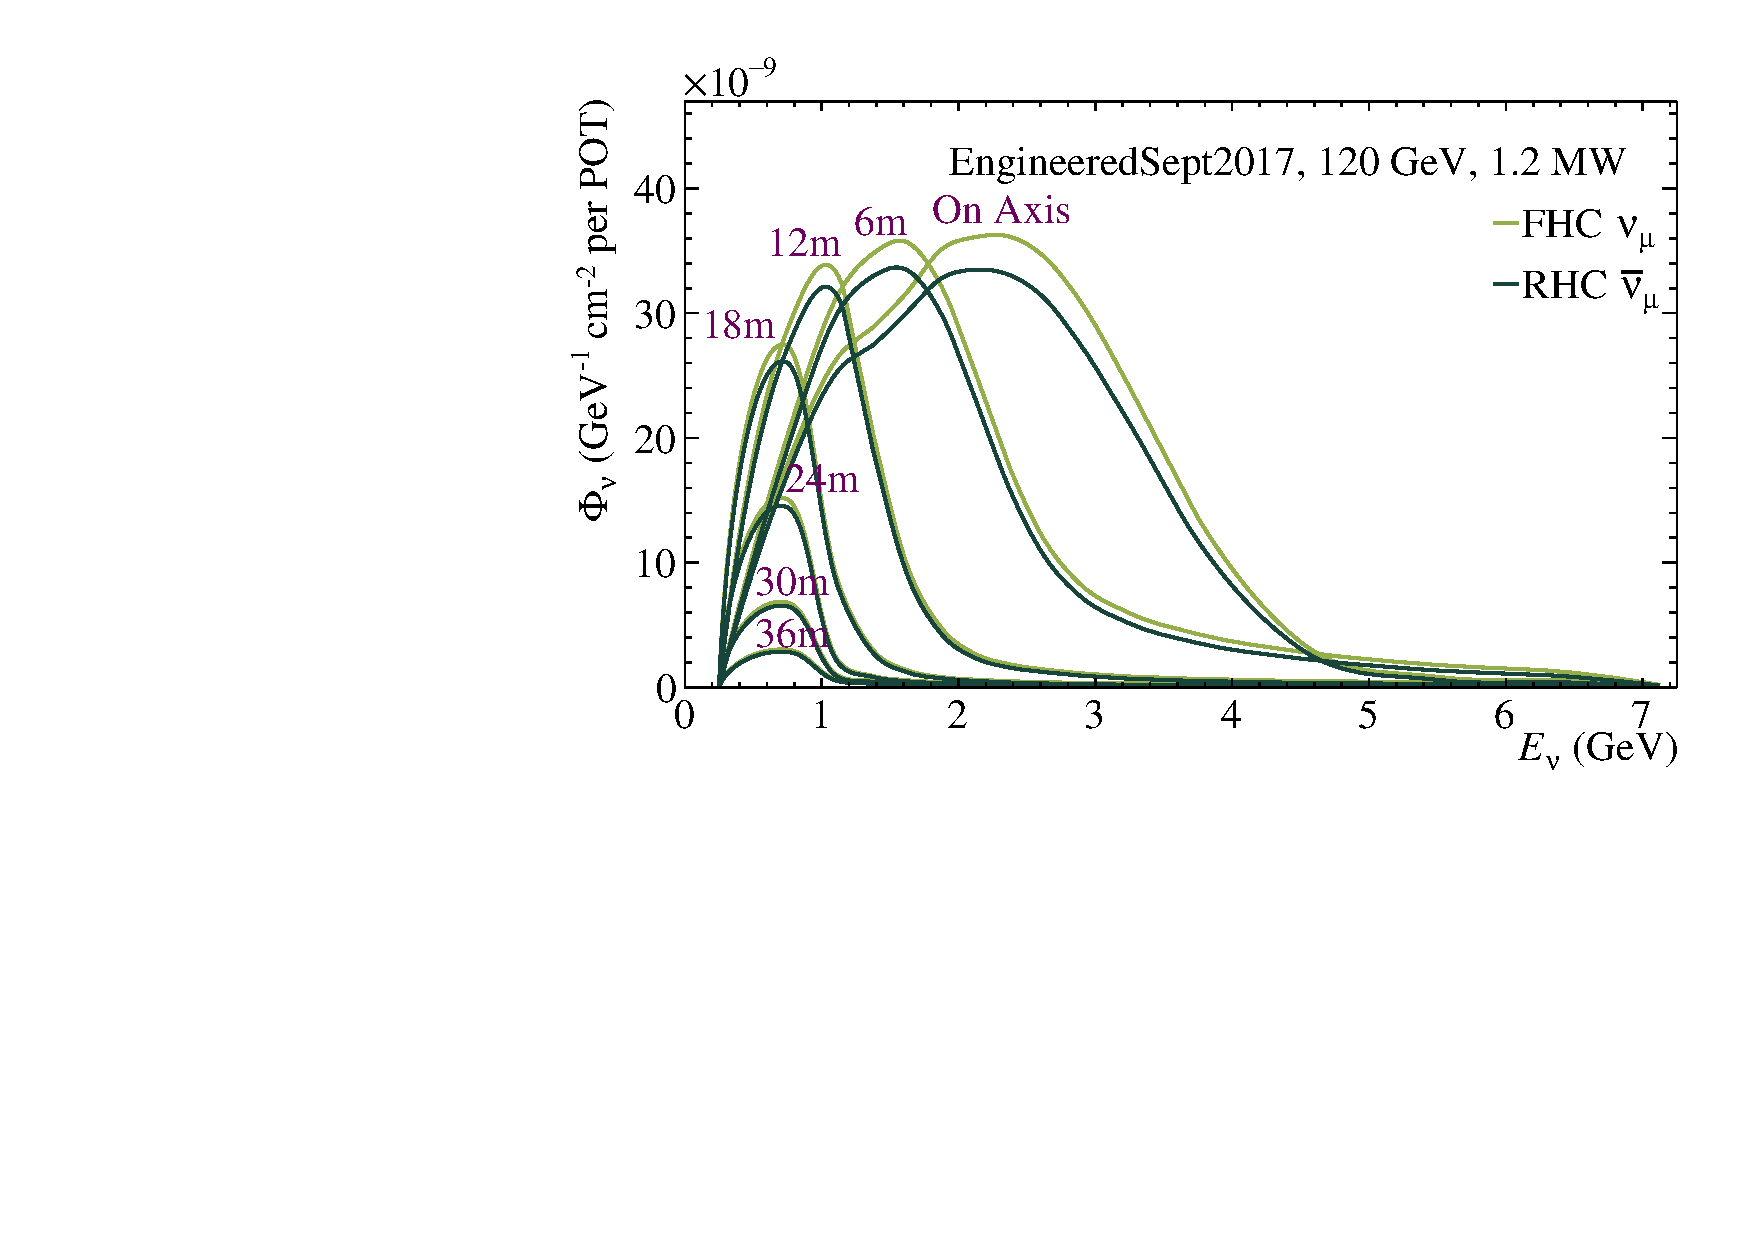
\includegraphics[width=0.45\textwidth]{OffAxisFluxes_1D}}
%    \label{fig:OffAxisFluxes_1D}
%  }
\end{dunefigure}

The same sources of systematic uncertainty which affect the on-axis spectra also modify the off-axis spectra.  Generally, the size of the off-axis uncertainties is comparable to the on-axis uncertainties and the uncertainties are highly correlated across off-axis and on-axis positions. Studies of extreme changes to horn positions and current indicate that the larger than expected shifts to the horn focusing elements (as has been historically seen in NuMI) would induce significant changes off-axis. Therefore, off-axis flux measurements are useful to diagnose beamline physics, and to further constrain flux uncertainties.
